% compress:  compresses the navigation bar                                      
% trans | handout:  restrict overlays
\documentclass[dvips,xcolor=cmyk]{beamer}
%\documentclass[pdftex,compress,xcolor=cmyk,trans]{beamer}

% % force compression of graphic objects?  I need to research this more, JJS
% 4/24/12
% \pdfminorversion=5
% \pdfcompresslevel=9
% \pdfobjcompresslevel=2

%% Packages
\usepackage{amsmath,amssymb}
\usepackage{enumerate}
%\usepackage{graphics}
\usepackage{array}
\usepackage{psfrag}
%\usepackage{subfigure}
\usepackage{graphicx}
\usepackage{subfig}
%\usepackage{movie15} % separate package with good integration with Beamer
\usepackage{sidecap}
\usepackage{caption}

%\usepackage{easymovie}             
\usepackage[normalem]{ulem}

\usepackage{natbib,natbibspacing}
\newcommand{\newblock}{}

%\usepackage{enumitem}

\usepackage{pstricks}
%\usepackage{tikz}
%\usetikzlibrary{positioning}
%\usetikzlibrary{calc}
\usepackage{nameref}
\usepackage{url}

\usepackage[T1]{fontenc}
\usepackage{arev}
\usepackage{type1cm}  

\usepackage{setspace}  

\captionsetup{font=scriptsize,labelfont=scriptsize}
%\setlength{\parindent}{0.3in}
%\setlength{\parskip}{0.1in}

% commands not needed for math

%% Set formatting to conform to NREL standards
% NREL "signature" colors
\definecolor{nrelblue}{cmyk}{1,0.44,0,0}
\definecolor{nrelyellow}{cmyk}{0,0.42,1,0.01}
\definecolor{nrelgreen}{cmyk}{0.56,0,1,0.27}
\definecolor{nrelred}{cmyk}{0,0.74,1,0.47}
\definecolor{nrelgray}{cmyk}{0.11,0.01,0,0.64}
% NREL "secondary" colors -- double check these !! JJS 4/21/12
\definecolor{nrellightblue}{cmyk}{0.9,0.11,0,0}
\definecolor{nrellightyellow}{cmyk}{0,0.24,94,0}
\definecolor{nrellightgreen}{cmyk}{0.50,0,1,0}
\definecolor{nrellightred}{cmyk}{0,0.79,1,0.11}
\definecolor{nrellightgray}{cmyk}{0.02,0,0,0.18}

\input basic.ltx
\def\directory{EPSF/}

% custom defined colors
\definecolor{foottextcolor}{named}{white}

% set beamer theme(s)
\usecolortheme[named=nrelblue]{structure}
% \usefonttheme[onlymath]{serif}  % use sans serif for text, but serif for
% math

\newlength{\lrmargin} % left and right margin width
\setlength{\lrmargin}{1em}
\setbeamersize{text margin left=\lrmargin}
\setbeamersize{text margin right=\lrmargin}

\setbeamertemplate{navigation symbols}{}  % gets rid of navigation symbols

% change the default footnote font size
\usepackage{etoolbox}
\makeatletter
\patchcmd{\@makefntext}{\insertfootnotetext{#1}}{\insertfootnotetext{\tiny#1}}{}{}
\makeatother

% define frame-title template
\setbeamertemplate{frametitle}
{
  \textbf{\Large \insertframetitle}
  \par
  \vspace{-0.5ex}
  \mbox{\hspace{-\lrmargin}\rule{\paperwidth}{0.2ex}}
}
\setbeamertemplate{footline}
{
  \colorbox{nrelblue}{\parbox{0.99\paperwidth}{
      \color{foottextcolor} \Tiny
      \hspace{\stretch{0.05}} NATIONAL RENEWABLE ENERGY LABORATORY \hfill
\textbf{\insertframenumber}\hspace{\stretch{0.1}} }}
}

% specify subitem to be a circle
\setbeamertemplate{itemize subitem}[circle]

%% define a ``listheader'' format
\newcommand{\listhead}[1]{{\color{nrelblue}\textbf{#1}}}
%\newcommand{\listhead}[1]{\textbf{#1}}

%% define a custom itemize environment with adjusted spacing
\newenvironment{myitemize}[1][]{\begin{itemize}[#1]\addtolength{\itemsep}{1ex}}{\end{itemize}}

\newcommand{\uvec}[1]{\bar{#1}}
\newcommand{\tens}[1]{\underline{\underline{#1}}}
\renewcommand{\vec}[1]{\underline{#1}}
\renewcommand{\skew}[1]{\widetilde{#1}}


\begin{document}

%
{\setbeamercolor{normal text}{fg=white,bg=nrelblue}
  \usebeamercolor[fg]{normal text}
\begin{frame}[plain]

\rput[tl](-0.2,2.2){

\includegraphics[width=0.2\textwidth,clip]{nrel_logo_white.eps}}

\rput[tl](3.4,2.1){\parbox{\textwidth}{
\textbf{Nonlinear Legendre Spectral \\
Finite Elements for Wind Turbine \\
Blade Dynamics} } }

\rput[tl](-0.5,1.0){
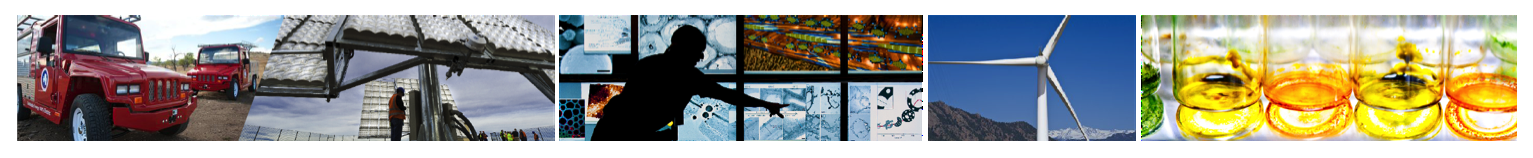
\includegraphics[width=1.1\textwidth,clip]{nrel_photo_bar.eps}
}

\rput[tl](2.0,-0.5){\parbox{\textwidth}{  \normalsize
Qi Wang$^1$,  Nick Johnson$^2$\\
Michael A.~Sprague$^1$, Jason Jonkman$^1$
}}

\rput[tl](2.0,-1.2){\parbox{0.8\textwidth}{\footnotesize
$^1$National Renewable Energy Laboratory\\
$^2$Colorado School of Mines \\
}}

\rput[tl](2.0,-1.8){\parbox{\textwidth}
{AIAA SciTech 2015\\Kissimmee, FL\\
5--9 January 2015}}

\rput[tl](0.0,-3.5){\parbox{\textwidth}{
{
\begin{spacing}{0.6}
\tiny NREL is a national laboratory of the U.S.\ Department of Energy,
Office of
Energy Efficiency and Renewable Energy, 
operated by the Alliance for Sustainable Energy, LLC.
\end{spacing}
}}} 

\psline[linewidth=1pt,linecolor=white](-1,-4.9)(8,20)

\psline[linewidth=1pt,linecolor=white](-1,-2.0)(11,20)    

 \end{frame}
}

%------------------------------------------------------------------------------
\begin{frame}{Motivation}
  \begin{itemize}
    \item
    Beam model currently used in FAST
    \begin{itemize}
      \item
      Euler-Bernoulli beam model with shortening effect
      \item
      Two degree-of-freedoms
      \item
      Assumed-mode method
    \end{itemize}
    \item
    Beam models used in other wind turbine tools
    \begin{itemize}
        \item
        Multibody-formulation
        \item
        Linear beam models
        \item
        Constraints introduced between linear beams to describe large deflections and rotations
        \item
        Finite element method
    \end{itemize}
  \end{itemize}
\end{frame}
%------------------------------------------------------------------------------



%------------------------------------------------------------------------------

\begin{frame}{Objective}
    \normalsize
    \begin{itemize}
    \item
    Objective: create efficient high-fidelity beam models for wind turbine blade analysis that can
      \begin{itemize}
          \item
          Capture geometrical nonlinearity systematically 
          \item
          Capture anisotropic and heterogeneous behavior of composite materials rigorously
          \item
          Modeling moving beams (translation and rotation)
          \item
          Achieve the speed of computational design without significant loss of accuracy comparing to the ultimate accuracy obtained by 3D nonlinear FEA
          \item
          Compatible with the FAST modularization framework
      \end{itemize}
    \end{itemize}
    \includegraphics[width=0.4\textwidth,clip=true]{figs/static_test.eps}
\hspace{0.05in}
\includegraphics[width=0.18\textwidth,clip=true]{figs/dyn_test.eps}

\rput[tl](7.6,2.5){\parbox{0.35\textwidth}{\small NWTC static and dynamic
blade tests showing typical large, elastic deflections.}}
\end{frame}
%------------------------------------------------------------------------------

%------------------------------------------------------------------------------
\begin{frame}{Approach}
  \begin{itemize}
    \item
    Implementation
    \begin{itemize}
      \item
      Geometrically Exact Beam Theory (GEBT) 
      \begin{itemize}
        \item
        \pause
        First proposed in 1973 \citep{Ressiner1973}
        \item
        \pause
        Extended to composite beams \citep{HodgesBeamBook}
        \item
        \pause
        Displacement-based implementation \citep{Dymore:2013}
        \item
        \pause
        Mixed implementation \citep{YuGEBT}
      \end{itemize}
      \item
      Legendre Spectral Finite Element (LSFE) \citep{Patera:1984}
      \begin{itemize}
          \item
          \pause
          A $p$-version high-order finite element 
          \item
          \pause
          Successfully applied to simulation of fluid dynamics, geophysics, elastodynamics
          \item
          \pause
          Limited usage in structural dynamics
      \end{itemize}
      \item
      FAST Modularization Framework \citep{Jonkman:2013}
      \begin{itemize}
          \item State-space formulation for tight-coupling scheme
          \item Time integrator for first-order PDEs
      \end{itemize}
    \end{itemize}
    \item
    Result: BeamDyn, which can be used as a structural module of FAST
  \end{itemize}
\end{frame}
%------------------------------------------------------------------------------

%------------------------------------------------------------------------------
\begin{frame}{GEBT}
\begin{itemize}
    \item Governing Equation
      \begin{align*} 
      \dot{\underline{h}} - \underline{F}^\prime &= \underline{f} \\
      \dot{\underline{g}} + \dot{\widetilde{u}} \underline{h} -
      \underline{M}^\prime - (\widetilde{x}_0^\prime + \widetilde{u}^\prime) \underline{F}
      &= \underline{m} 
      \end{align*}
    
    \item Constitutive Equation
    \begin{columns}[c]
      \column{2.0 in}
      
      \begin{align*}
      \begin{Bmatrix} \underline{h} \\ \underline{g} \end{Bmatrix} &=
      \underline{\underline{\mathcal{M}}} \begin{Bmatrix} \dot{\underline{u}} \\
      \underline{\omega} \end{Bmatrix} \\
      \begin{Bmatrix} \underline{F} \\ \underline{M} \end{Bmatrix} &=
      \underline{\underline{\mathcal{C}}} \begin{Bmatrix} \underline{\epsilon} \\
      \underline{\kappa} \end{Bmatrix} 
      \end{align*}
      \column{2.0 in}
      \begin{itemize}
        \scriptsize
        \pause
        \item
        $\ten{\mathcal{M}}$ and $\ten{\mathcal{C}}$ are $6 \times 6$ sectional mass and stiffness matrices, respcetively \pause
        \item
        Elastic couplings are captured \pause
        \item
        Timoshenko-like beam model
      \end{itemize}
      
      \end{columns}

    \item Strain Measures
    
    \begin{columns}[c]
    \column{2.0 in}
      \begin{equation*}
      \label{1DStrain}
      \begin{Bmatrix}
          \vec{\epsilon} \\
          \vec{\kappa}
      \end{Bmatrix}
      =
      \begin{Bmatrix}
          \vec{x}^\prime_0 + \vec{u}^\prime - (\tens{R} ~\tens{R}_0) \bar{\imath}_1 \\
          \vec{k} 
      \end{Bmatrix}
      \end{equation*}   
      
      \column{2.0 in}
        \begin{itemize}
        \scriptsize
          \pause
          \item
          Geometrically exact: deformed beam geometry is represented exactly
          \pause
          \item 
          Small strains
        \end{itemize}
      \end{columns}
    \end{itemize}

\end{frame}
%------------------------------------------------------------------------------

%------------------------------------------------------------------------------
\begin{frame}[shrink=10]{State-space Formulation}

\begin{itemize}
    \item Governing Equation
    \begin{equation*}
        \label{CompactForm2}
        \underline{\underline{\mathfrak{M}}}~ \underline{a} + f(\underline{q},\underline{v},t) = 0
    \end{equation*} 
    \begin{columns}[c]
    \column{1.5 in}
    \begin{equation*}     
        \underline{q}^T = \left[ \underline{u}^T~~\underline{p}^T \right]
    \end{equation*} 
        
    \column{1.5 in}
     \begin{equation*}
        \underline{v}^T = \left[\underline{\dot{u}}^T~~\underline{\omega}^T \right]
    \end{equation*}
    
    \column{1.5 in}
    \begin{equation*}
        \underline{a}^T = \left[ \ddot{\underline{u}}^T~~\dot{\underline{\omega}}^T \right]
    \end{equation*}
    \end{columns}    
    
    \item State-Space Form
    \begin{equation*}
        \label{StateSpaceGov-1}
        \tens{A} ~\dot{\hat{\vec{x}}}(t) = \mathfrak{f}(\hat{\vec{x}}(t),t)
    \end{equation*}
    
    \begin{columns}[c]
    \column{2.0 in}
    \begin{equation*}
        \label{StateSpaceX}
        \vec{x}(t) \equiv \begin{Bmatrix}
        \vec{q}(t) \\
        \vec{v}(t)
        \end{Bmatrix} 
    \end{equation*}
    \begin{equation*}
         \tens{D} (\hat{\vec{x}}(t)) &= \int_0^l \tens{N}^T \begin{bmatrix}
        \tens{I}_3 & \tens{0} \\
        \tens{0} & \tens{H}
        \end{bmatrix} 
        \tens{N}~dx_1
    \end{equation*}
    
    \column{2.0 in}
    \begin{equation*}
         \tens{A} (\hat{\vec{x}}(t)) &= \begin{bmatrix}
        \tens{D} & \tens{0} \\
        \tens{0} & \tens{M}
        \end{bmatrix}
    \end{equation*} 
    \begin{equation*}
    \mathfrak{f}(\hat{\vec{x}}(t),t) &=  \begin{Bmatrix}
    \int_0^l \tens{N}^T \vec{v}~dx_1 \\
    \vec{F}(\hat{\vec{x}}(t),t)
    \end{Bmatrix}
    \end{equation*}
    
    \end{columns}
    
    \item Second-order Adams-Moulton (AM2)
    \begin{equation*}
    \label{AM2-Govn}
    \tens{A}_{k+1} (\hat{\vec{x}}_{k+1}-\hat{\vec{x}}_{k} - \frac{\Delta t}{2} \vec{\dot{\hat{x}}}_k) =  \frac{\Delta t}{2} \mathfrak{f}(\hat{\vec{x}}_{k+1},t_{k+1})  
    \end{equation*}
      
\end{itemize}

\end{frame}
%------------------------------------------------------------------------------

%------------------------------------------------------------------------------
\begin{frame}{Legendre Spectral Finite Elements}
\normalsize

LSFE methods combine the geometric flexibility of
the FE method with the accuracy of global spectral methods.
%
\begin{itemize}
%
   \item Solution improved through increased basis polynomial order
($p$-refinement)
%
    \item LSFEs employ Lagrangian interpolant shape functions with nodes at
Gauss-Lobatto-Legendre (GLL) points 
%    \item Early SFEs employed Chebyshev-based shape functions; largely
%abandoned in favor of more straight-forward and efficient Legendre-based
%elements
%
  \item \textit{Exponential} convergence rates for sufficiently
smooth solutions
%
%  \item SFEs should not be confused with what are known as \textit{spectral
%elements}, or \textit{modal spectral elements},
%in the structural analysis community (\eg, Doyle 1997)
\end{itemize}

\begin{figure}[h!tp]
   \psfrag{note}[][]{$p$ refine}
   \psfrag{p1}[][]{$N=1$}
   \psfrag{p2}[][]{$N=4$}
   \includegraphics[width=0.5\textwidth,clip]{figs/refine.eps}
\end{figure}

\end{frame}

%------------------------------------------------------------------------------

%------------------------------------------------------------------------------
\begin{frame}{Example 1: Initially Twisted Beam}
    \begin{itemize}
    \item Sketch of Initially Twisted Beam
    \begin{center}
    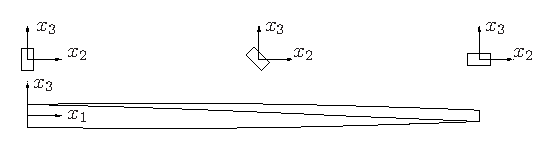
\includegraphics[width=3.0in]{EPSF/twist_beam.eps}
    \end{center}
    \item Result
    \begin{table}
    \caption{\label{E1u} Comparison of tip displacements of an initially twisted beam} 
    \begin{center} 
        \begin{tabular}{| l | l | l | l | l | l | l |}
    	    \hline
    	        & $u_1$ (m) & $u_2$ (m) & $u_3$ (m)  \\ \hline
    	BeamDyn  & -1.132727     & -1.715123       & -3.578671      \\  \hline
    	ANSYS   & -1.134192     & -1.714467      & -3.584232     \\ \hline
    	Percent Error   & 0.129\%     & 0.038\%      & 0.155\%     \\ \hline
    \end{tabular}
\end{center}
\end{table} 
    \end{itemize}
\end{frame}
%------------------------------------------------------------------------------

%------------------------------------------------------------------------------
\begin{frame}{Example 1: Initially Curved Beam}
    \begin{itemize}
    \item Sketch of Initially Curved Beam
    \begin{center}
    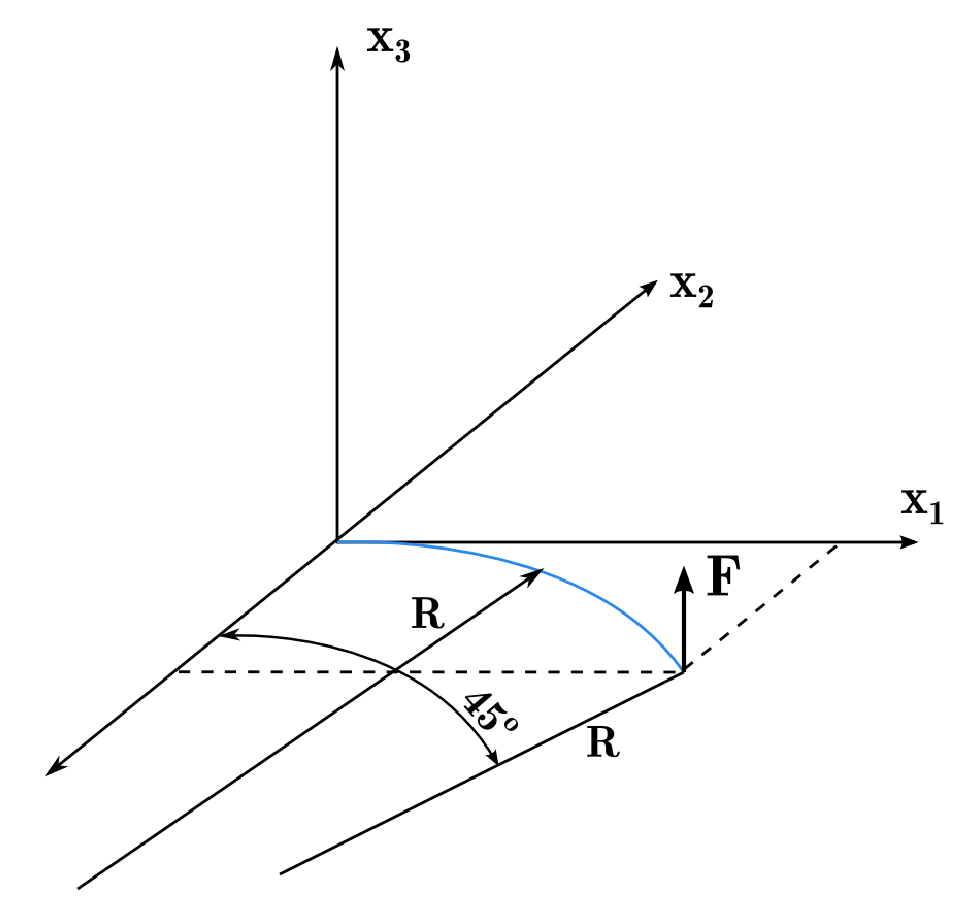
\includegraphics[width=1.5in]{EPSF/E1Curved.eps}
    \end{center}
    \item Result
    \scriptsize
    \begin{table}
\caption{\label{E1CurvedDisp} Comparison of tip displacements of an initially curved beam } 
\begin{center}
    \begin{tabular}{| l | l | l | l | l | l | l |}
    	\hline
    	        & $u_1$ (inches) & $u_2$ (inches) & $u_3$ (inches)  \\ \hline
    	BeamDyn (one LSFE) & -23.7     & 13.5       & 53.4      \\  \hline
    	Bathe-Bolourchi \cite{Bathe1979}   & -23.5     & 13.4       & 53.4     \\ \hline
    \end{tabular}
\end{center}
\end{table} 
    \end{itemize}
\end{frame}
%------------------------------------------------------------------------------

%------------------------------------------------------------------------------
\begin{frame}{Example 2: CX-100}
\begin{itemize}
\item Sketch of CX-100
    \begin{columns}[c]
    \column{2.0in}
     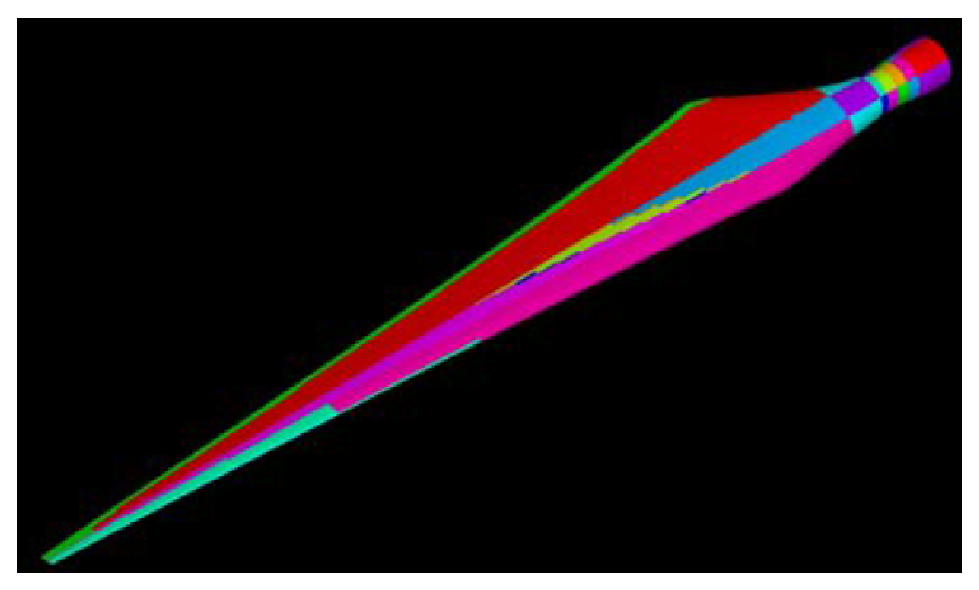
\includegraphics[width=2.0in]{EPSF/CX100Sketch.eps}
     \column{2.0in}
      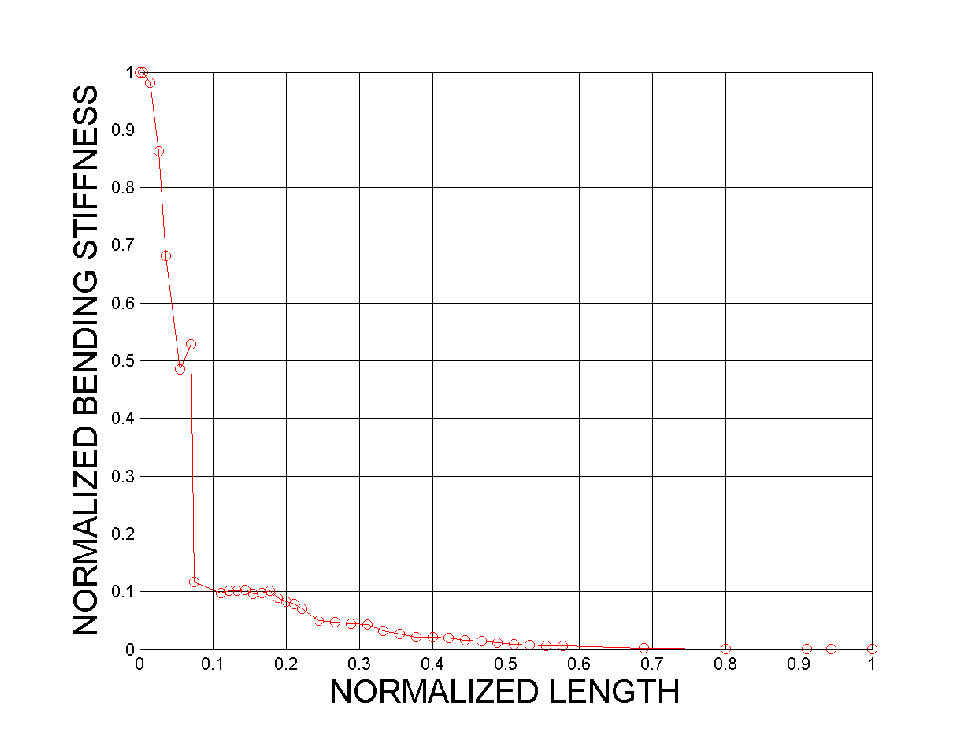
\includegraphics[width=2.0in]{EPSF/normalized1.eps}
    \end{columns}
    
\item Sectional Properties at 2.2 m
    \scriptsize
    \begin{align*}
C =10^3 \times \begin{bmatrix}
	193,000 & -75.4   & 12.2   & -75.2  & -1970    & -3500    \\
	-75.4  & 19,500 & 4,760   & 62.6  & 67.3    & 11.3    \\
	12.2  & 4,760   & 7,210 & -450  & 17.0    & 2.68    \\
	-75.2  & 62.6   & -450   & 518 & 1.66    & -1.11    \\
	-1,970  & 67.3   & 17.0   & 1.66  & 2,280 & -879    \\
	-3,500  & 11.6   & 2.68   & -1.11  & -875    & 4,240
\end{bmatrix}
\end{align*}
\end{itemize}
\end{frame}
%------------------------------------------------------------------------------

%------------------------------------------------------------------------------
\begin{frame}{Example 2: CX-100 (Continued)}
\begin{itemize}
\begin{columns}[c]
    \column{2.0 in}
    \item Static Test Configuration
    \begin{center}
     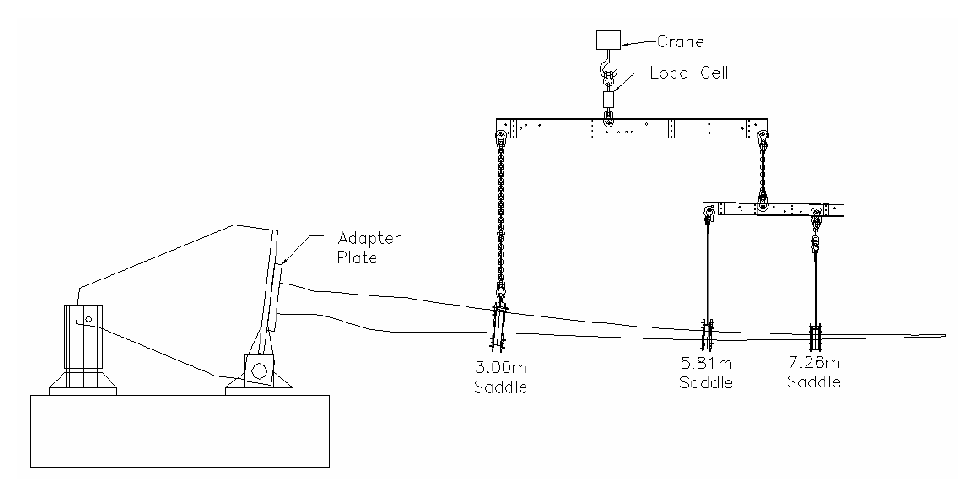
\includegraphics[width=2.4in]{EPSF/CX100Setup.eps}
     \end{center}
     
     \column{2.0 in}
     \item Deflection
     \begin{center}
     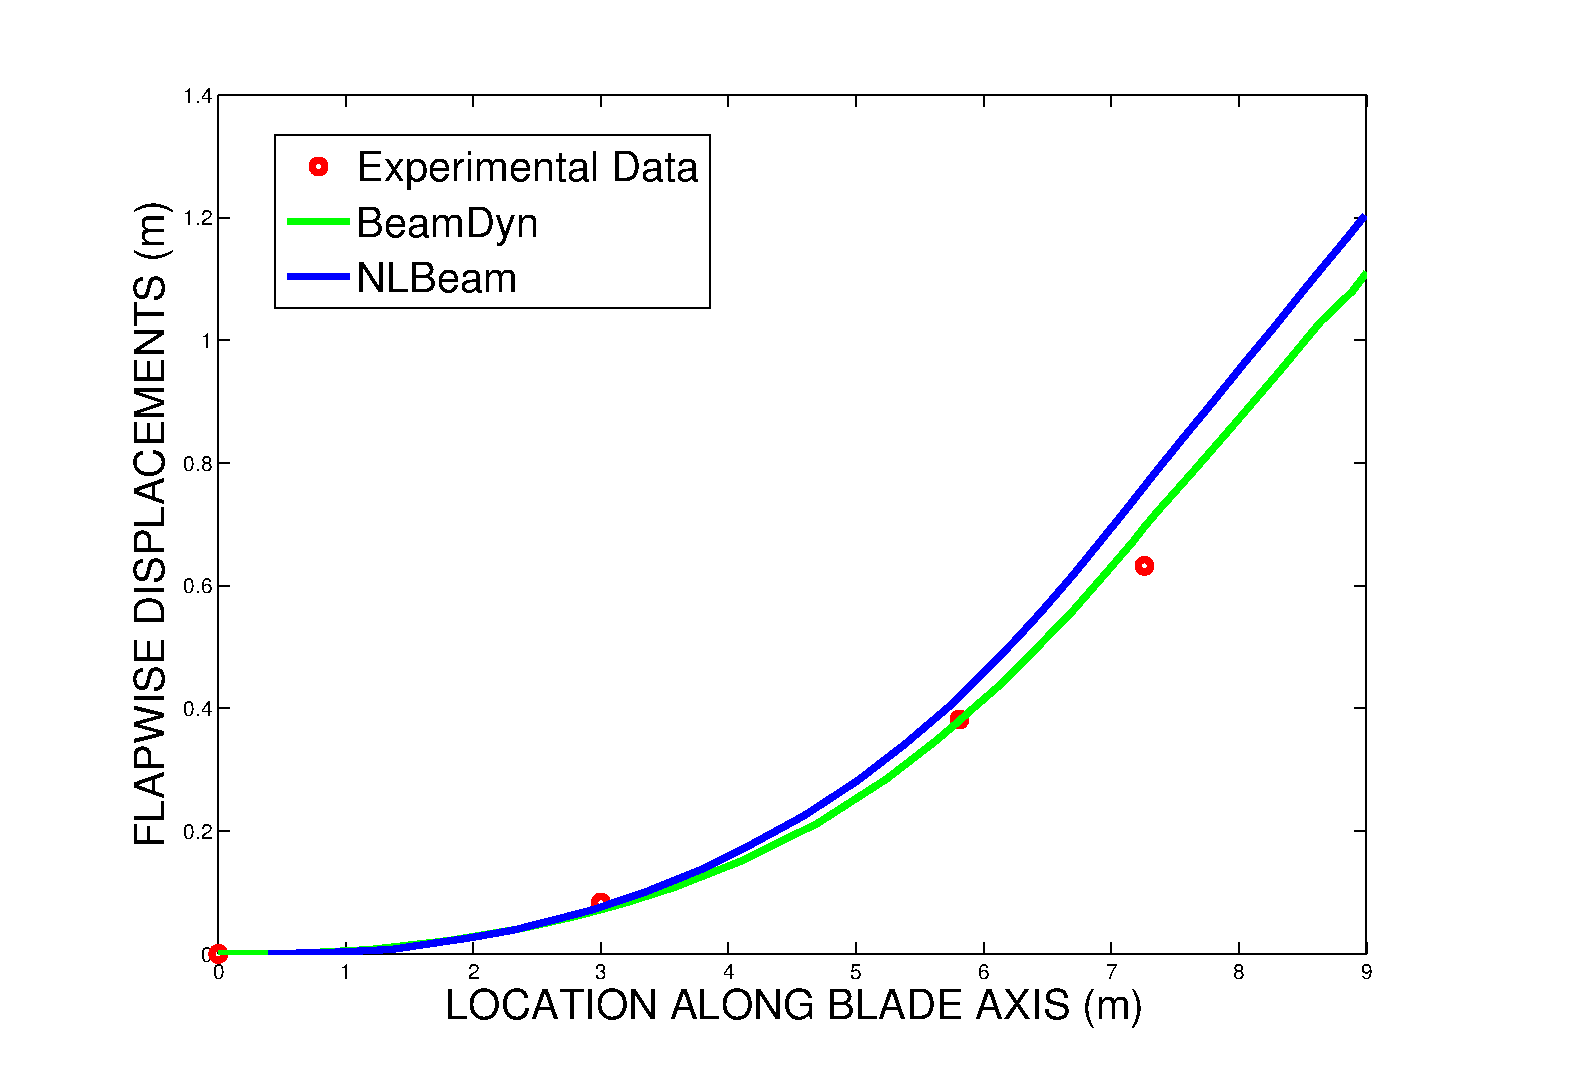
\includegraphics[width=2.0in]{EPSF/CX100Disp_New.eps}
     \end{center}
\end{columns}
\end{itemize}
\scriptsize
\begin{table}
\caption{\label{CX100Results}Experimental and BeamDyn simulation results for the CX-100 static test  } 
\begin{center}
    \begin{tabular}{| l | l | l | l |}
    	\hline
    	             & $u_3$ at saddle \#1 (m) & $u_3$ at saddle \#2 (m) & $u_3$ at saddle \#3 (m) \\ \hline
    	Experimental & 0.083530             & 0.381996               & 0.632460             \\ \hline
    	BeamDyn      & 0.072056               & 0.381074                & 0.698850           \\ \hline
    	    	Percent Error      &        13.74\%        & 0.24\%                & 10.5\%           \\ \hline
    \end{tabular}
\end{center}
\end{table} 
\end{frame}
%------------------------------------------------------------------------------

%------------------------------------------------------------------------------
\begin{frame}{Example 2: Convergence Study}
\begin{itemize}
\begin{columns}[c]
    \column{2.0 in}
    \item Validation
    \begin{center}
     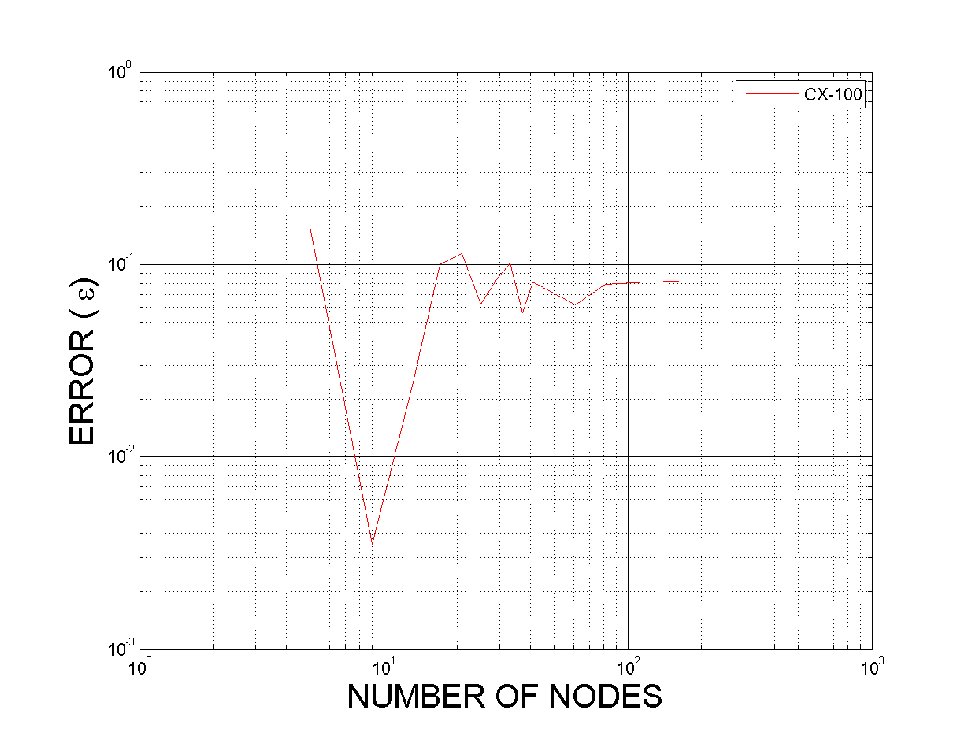
\includegraphics[width=2.2in]{EPSF/CX100conv3.eps}
     \end{center}
     
     \column{2.0 in}
     \item Verification
     \begin{center}
     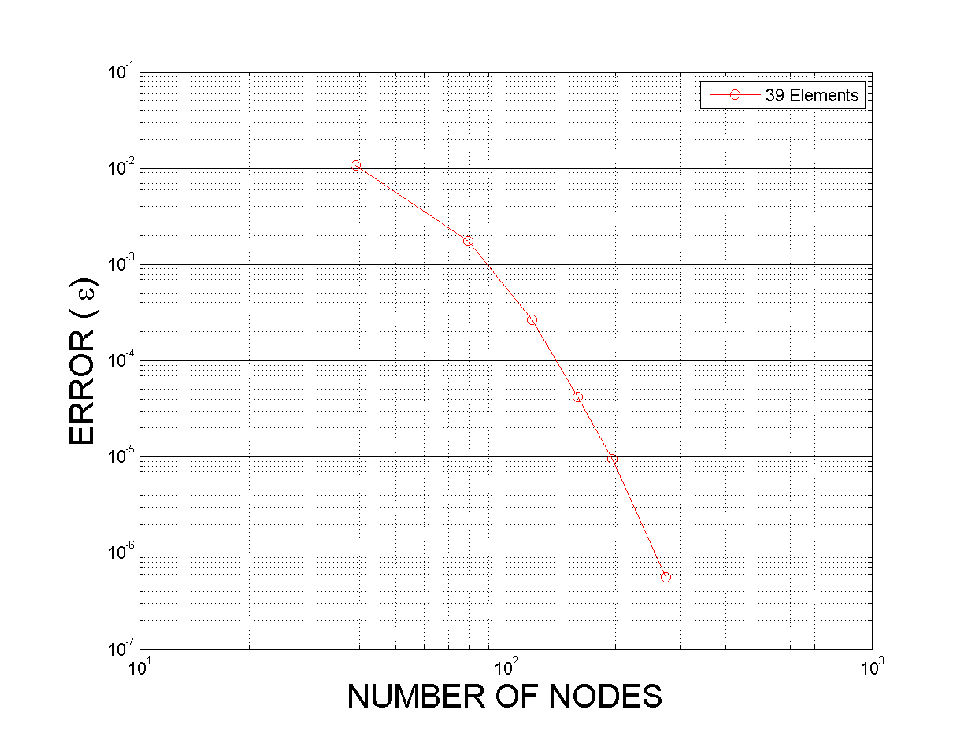
\includegraphics[width=2.2in]{EPSF/CX100elem2.eps}
     \end{center}
\end{columns}

\begin{itemize}
    \pause
    \item Sharp gradients in sectional properties
    \item Erratic data
\end{itemize}

\end{itemize}
\end{frame}
%------------------------------------------------------------------------------

%------------------------------------------------------------------------------
\begin{frame}{Example 3: Damping Effect}
\begin{itemize}
    \item Cantilever Beam Under Impulsive Load
    \begin{center}
     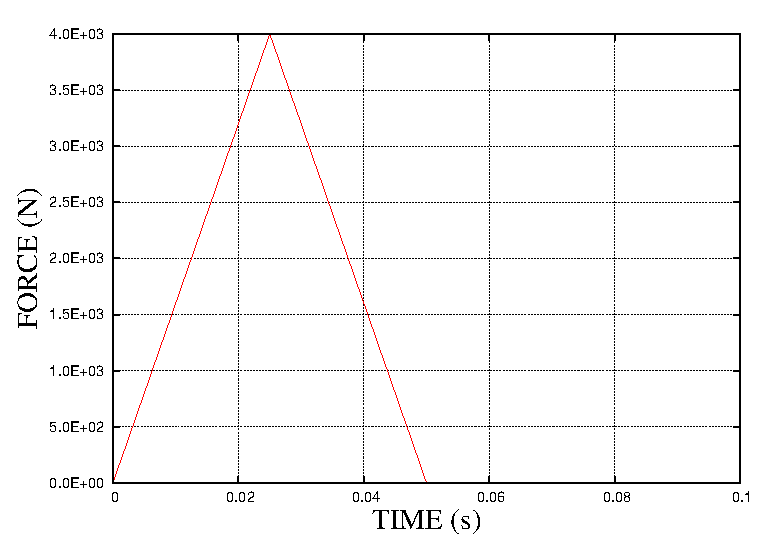
\includegraphics[width=2.2in]{EPSF/AM2_Excitation.eps}
     \end{center}  
     
     \pause
     \item Viscous Damping
     \begin{equation*}
   \label{Damping}
   \vec{f}_d = \tens{\mu}~ \tens{\mathcal{C}} \begin{Bmatrix}
   \dot{\epsilon} \\
   \dot{\kappa}
   \end{Bmatrix}
\end{equation*}

   \item RMS Error
   \begin{equation*}
\varepsilon_{RMS}=\sqrt{\frac{\sum_{k=0}^{n_{max}}[u_3^k-u_b(t^k)]^2}{\sum_{k=0}^{n_{max}}[u_b(t^k)]^2}}
\label{RMSdefi}
\end{equation*}
\end{itemize}
\end{frame}
%------------------------------------------------------------------------------

%------------------------------------------------------------------------------
\begin{frame}{Example 3: Root forces and moments}
\begin{itemize}
    \begin{columns}[c]
        \column{1.5in}
        \item $u_1$\\
        \linebreak[4]\\
          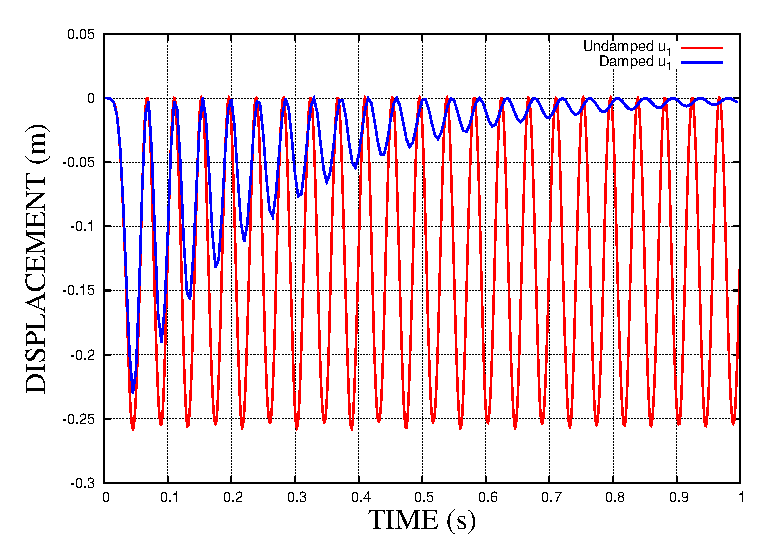
\includegraphics[width=1.5in]{EPSF/AM2_u1.eps}\\
          \item $p_1$\\
          \linebreak[4]
           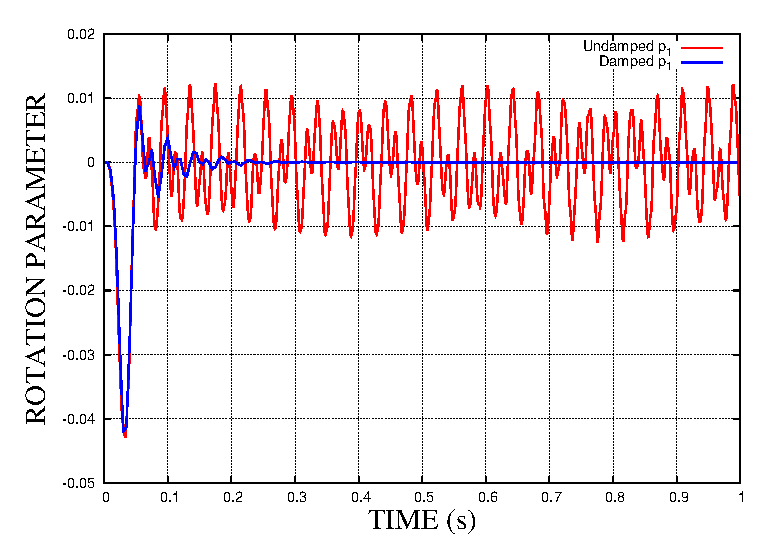
\includegraphics[width=1.5in]{EPSF/AM2_p1.eps}
         \column{1.5in} 
         \item $u_2$\\
        \linebreak[4]
           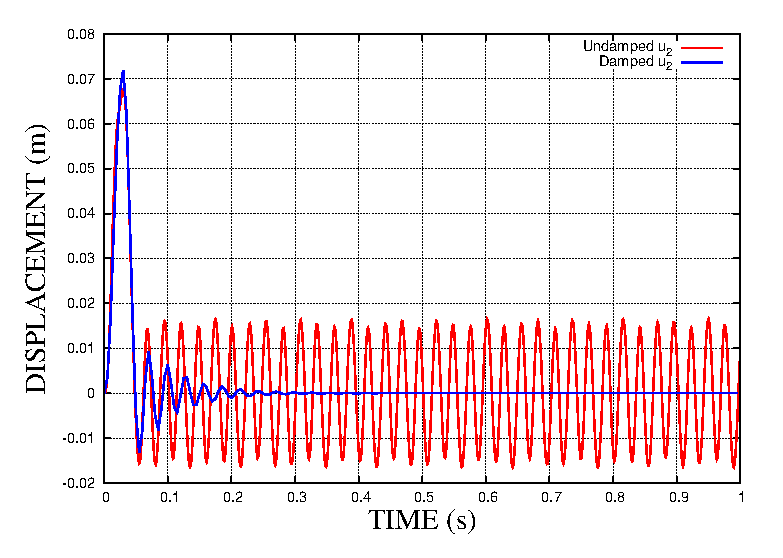
\includegraphics[width=1.5in]{EPSF/AM2_u2.eps}\\
          \item $p_2$\\
          \linebreak[4]
           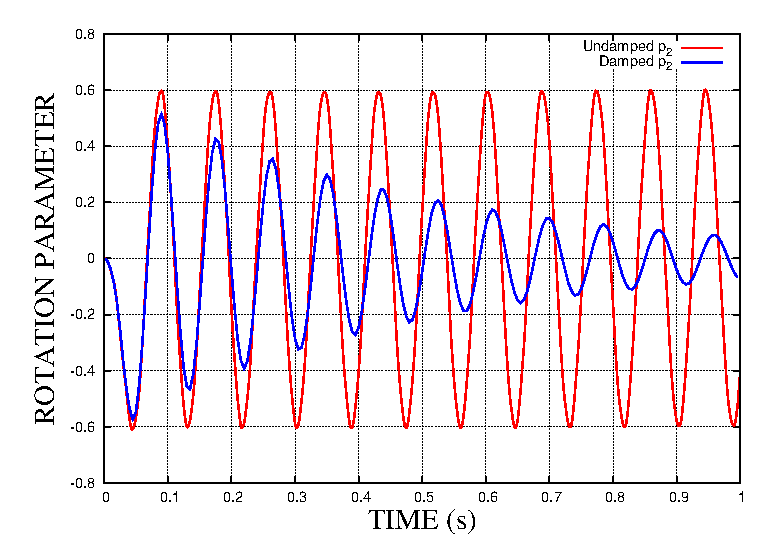
\includegraphics[width=1.5in]{EPSF/AM2_p2.eps} 
           \column{1.5in} 
           \item $u_3$\\
        \linebreak[4]
           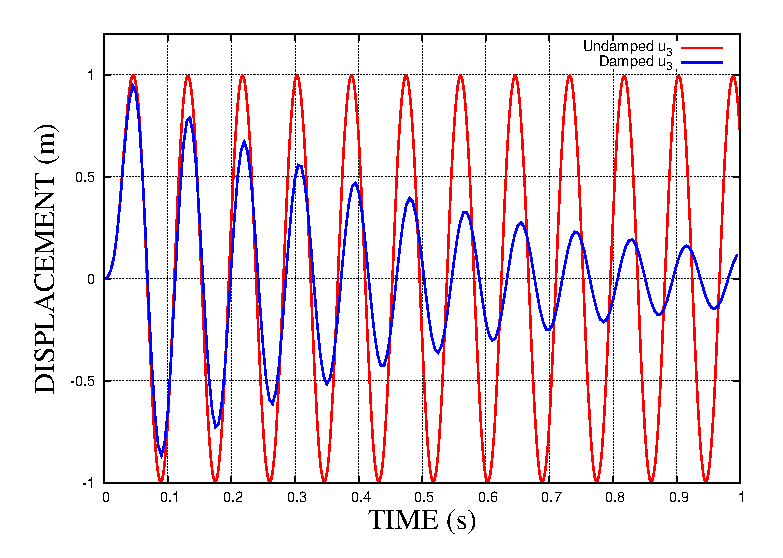
\includegraphics[width=1.5in]{EPSF/AM2_u3.eps}\\
          \item $p_3$\\
          \linebreak[4]
           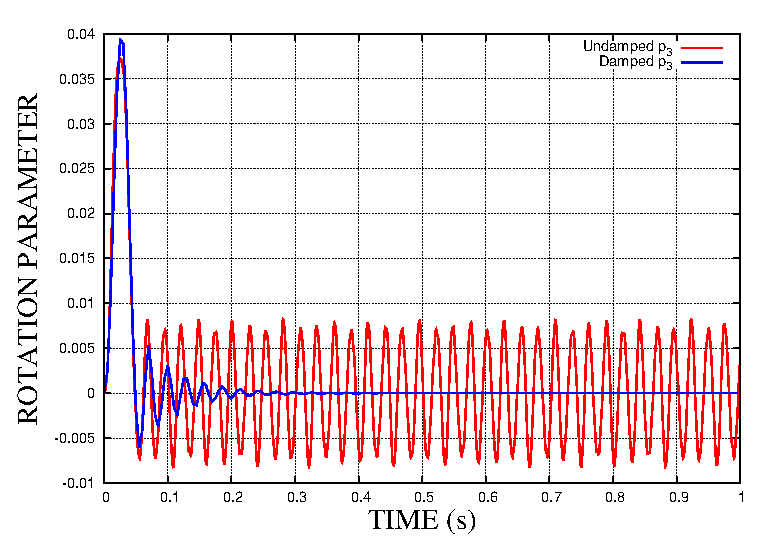
\includegraphics[width=1.5in]{EPSF/AM2_p3.eps}  
    \end{columns}
    
\end{itemize}
\end{frame}
%------------------------------------------------------------------------------


%------------------------------------------------------------------------------
\begin{frame}{Example 4: NREL 5-MW Blade}
\begin{itemize}
    \pause
    \item NREL 5-MW Blade; Cantilevered at root
    \pause
    \item White noise force applied at the free tip along flap direction
    \pause
    \item Time History of Applied Force
    \begin{center}
     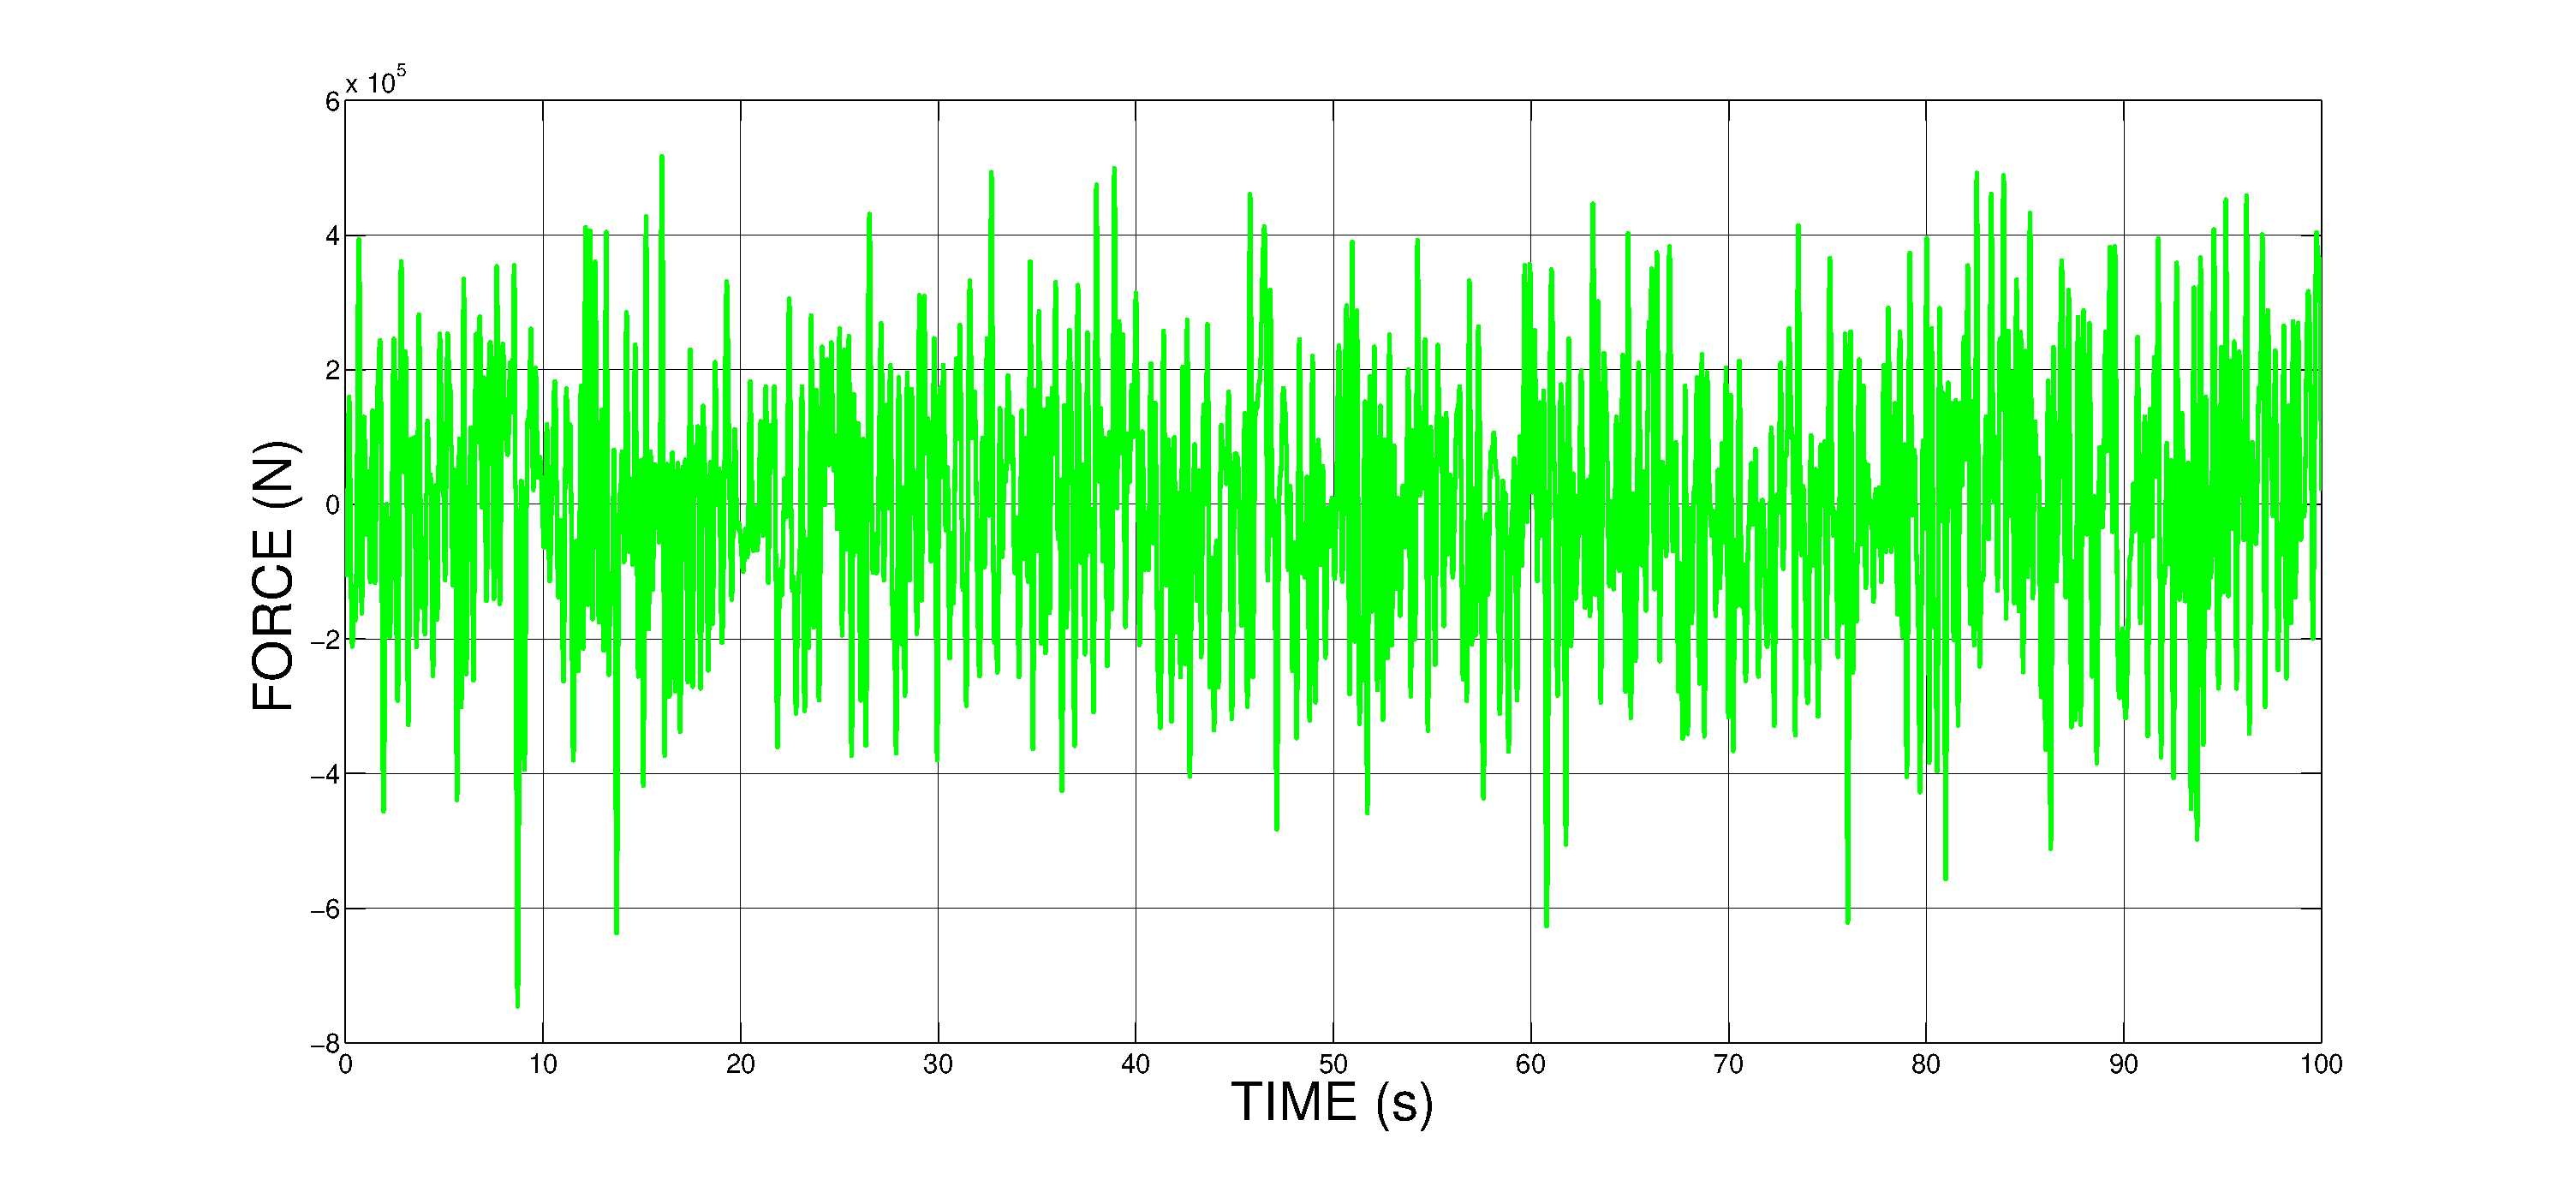
\includegraphics[width=2.2in]{EPSF/5MW_Flap_Force_Final.eps}
     \end{center}  
     \pause
      \item PSD of Applied Force
    \begin{center}
     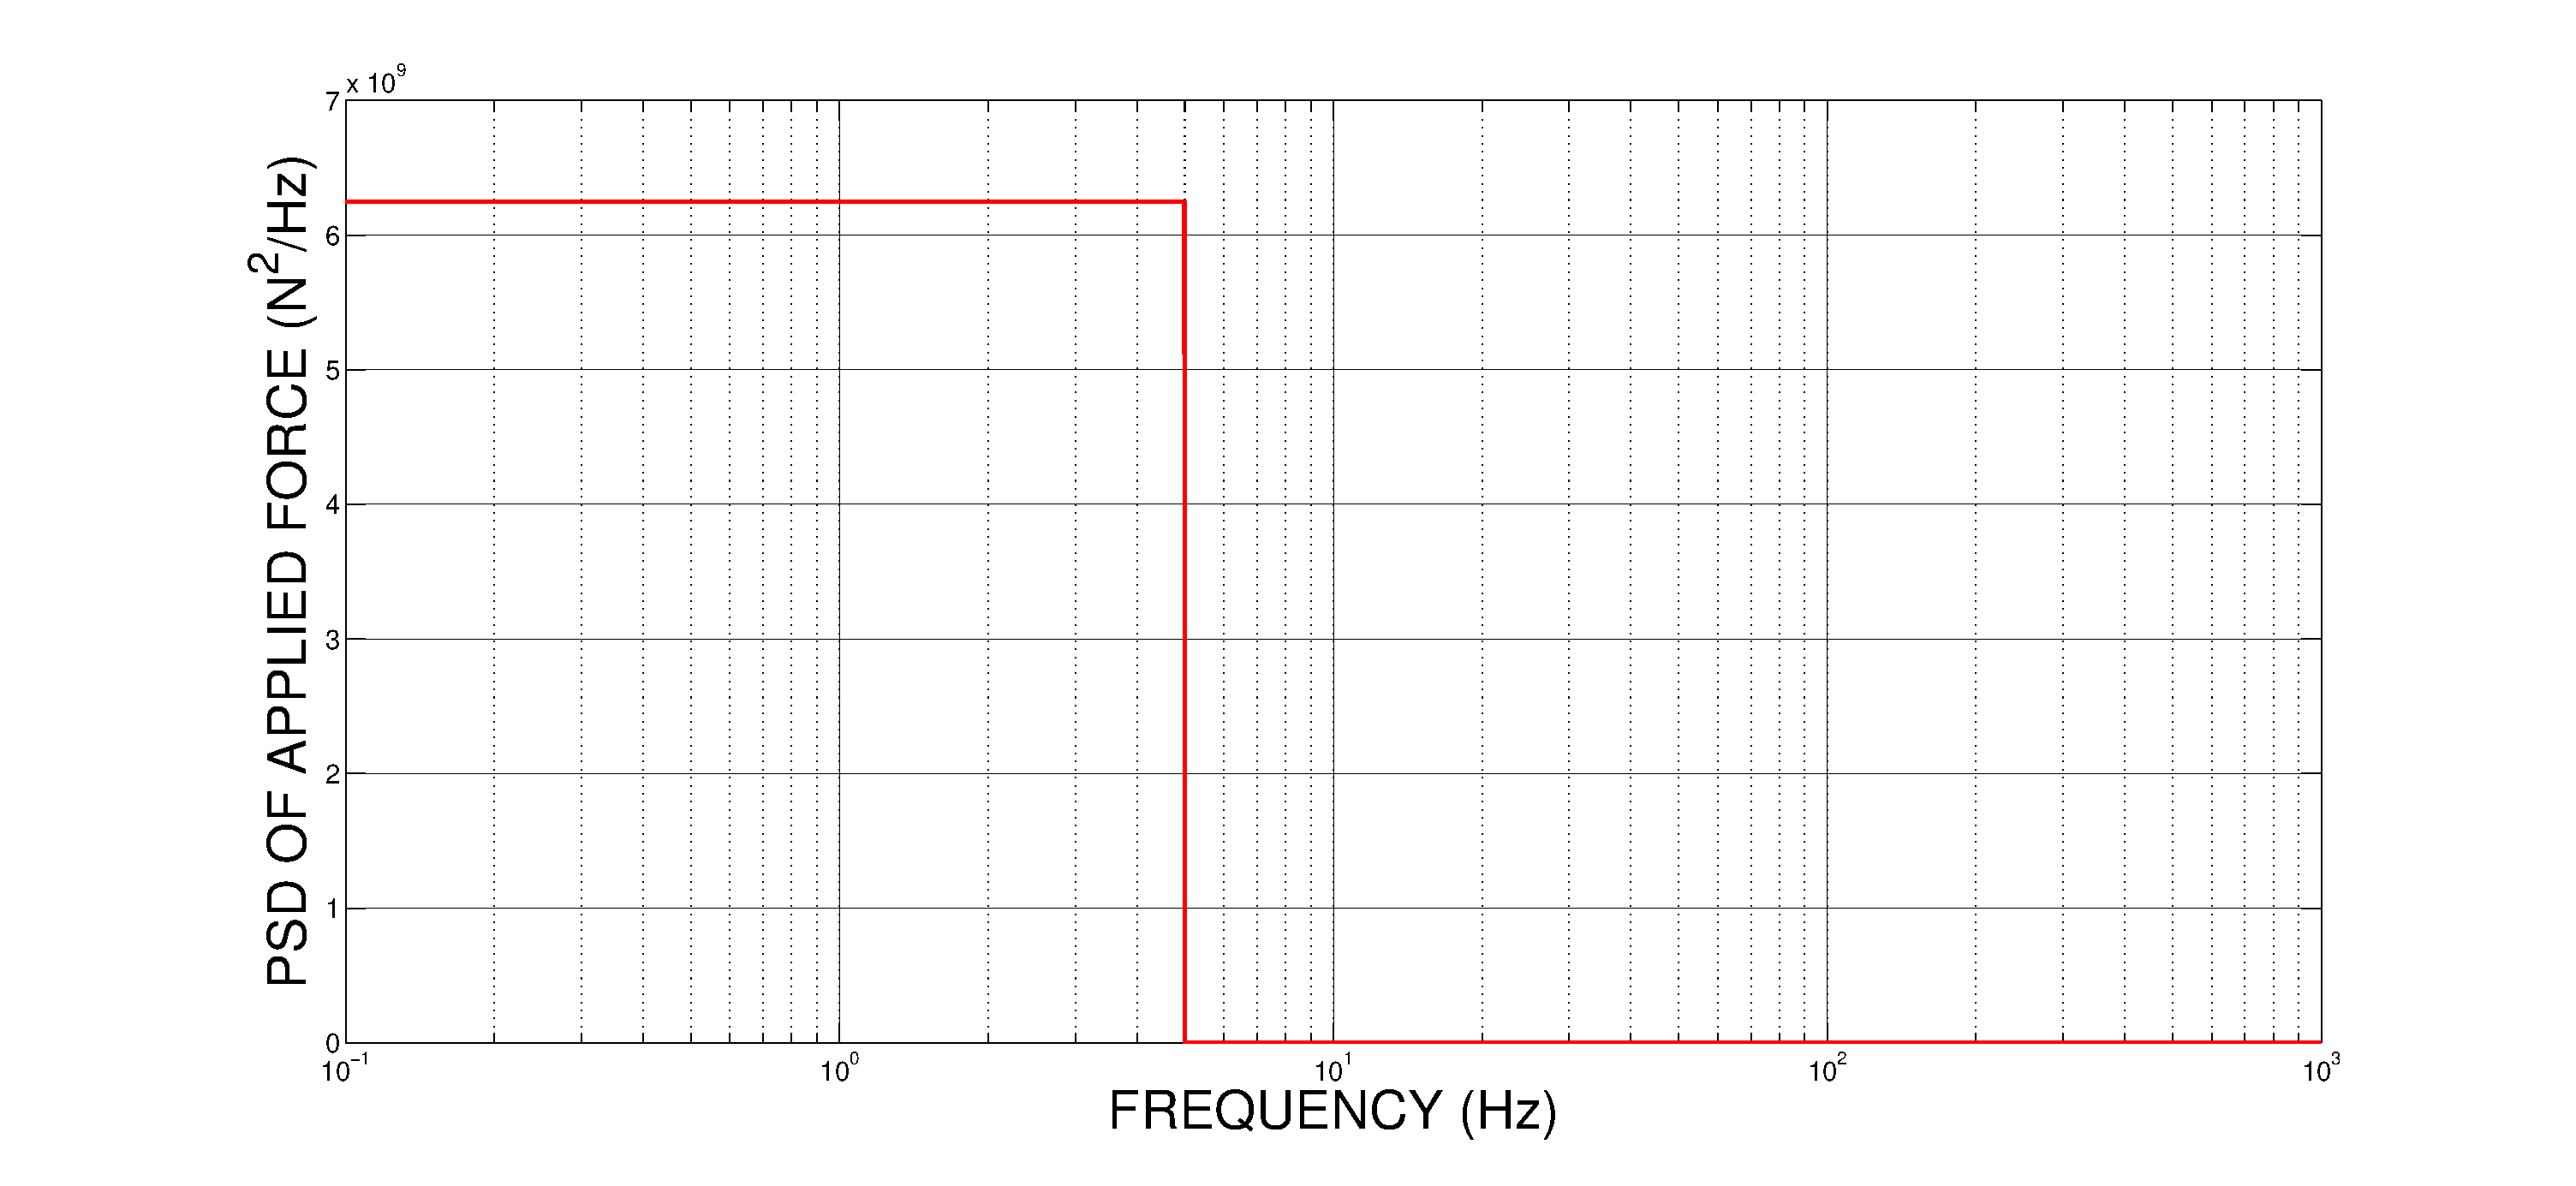
\includegraphics[width=2.2in]{EPSF/5MW_Flap_Force_PSD_Final.eps}
     \end{center}  
\end{itemize}
\end{frame}
%------------------------------------------------------------------------------

%------------------------------------------------------------------------------
\begin{frame}{Example 4: NREL 5-MW Blade (Continued)}
\begin{itemize}
   \begin{columns}[c]
   \column{2.0 in}
    \pause
    \item Flapwise Response
     \begin{center}
     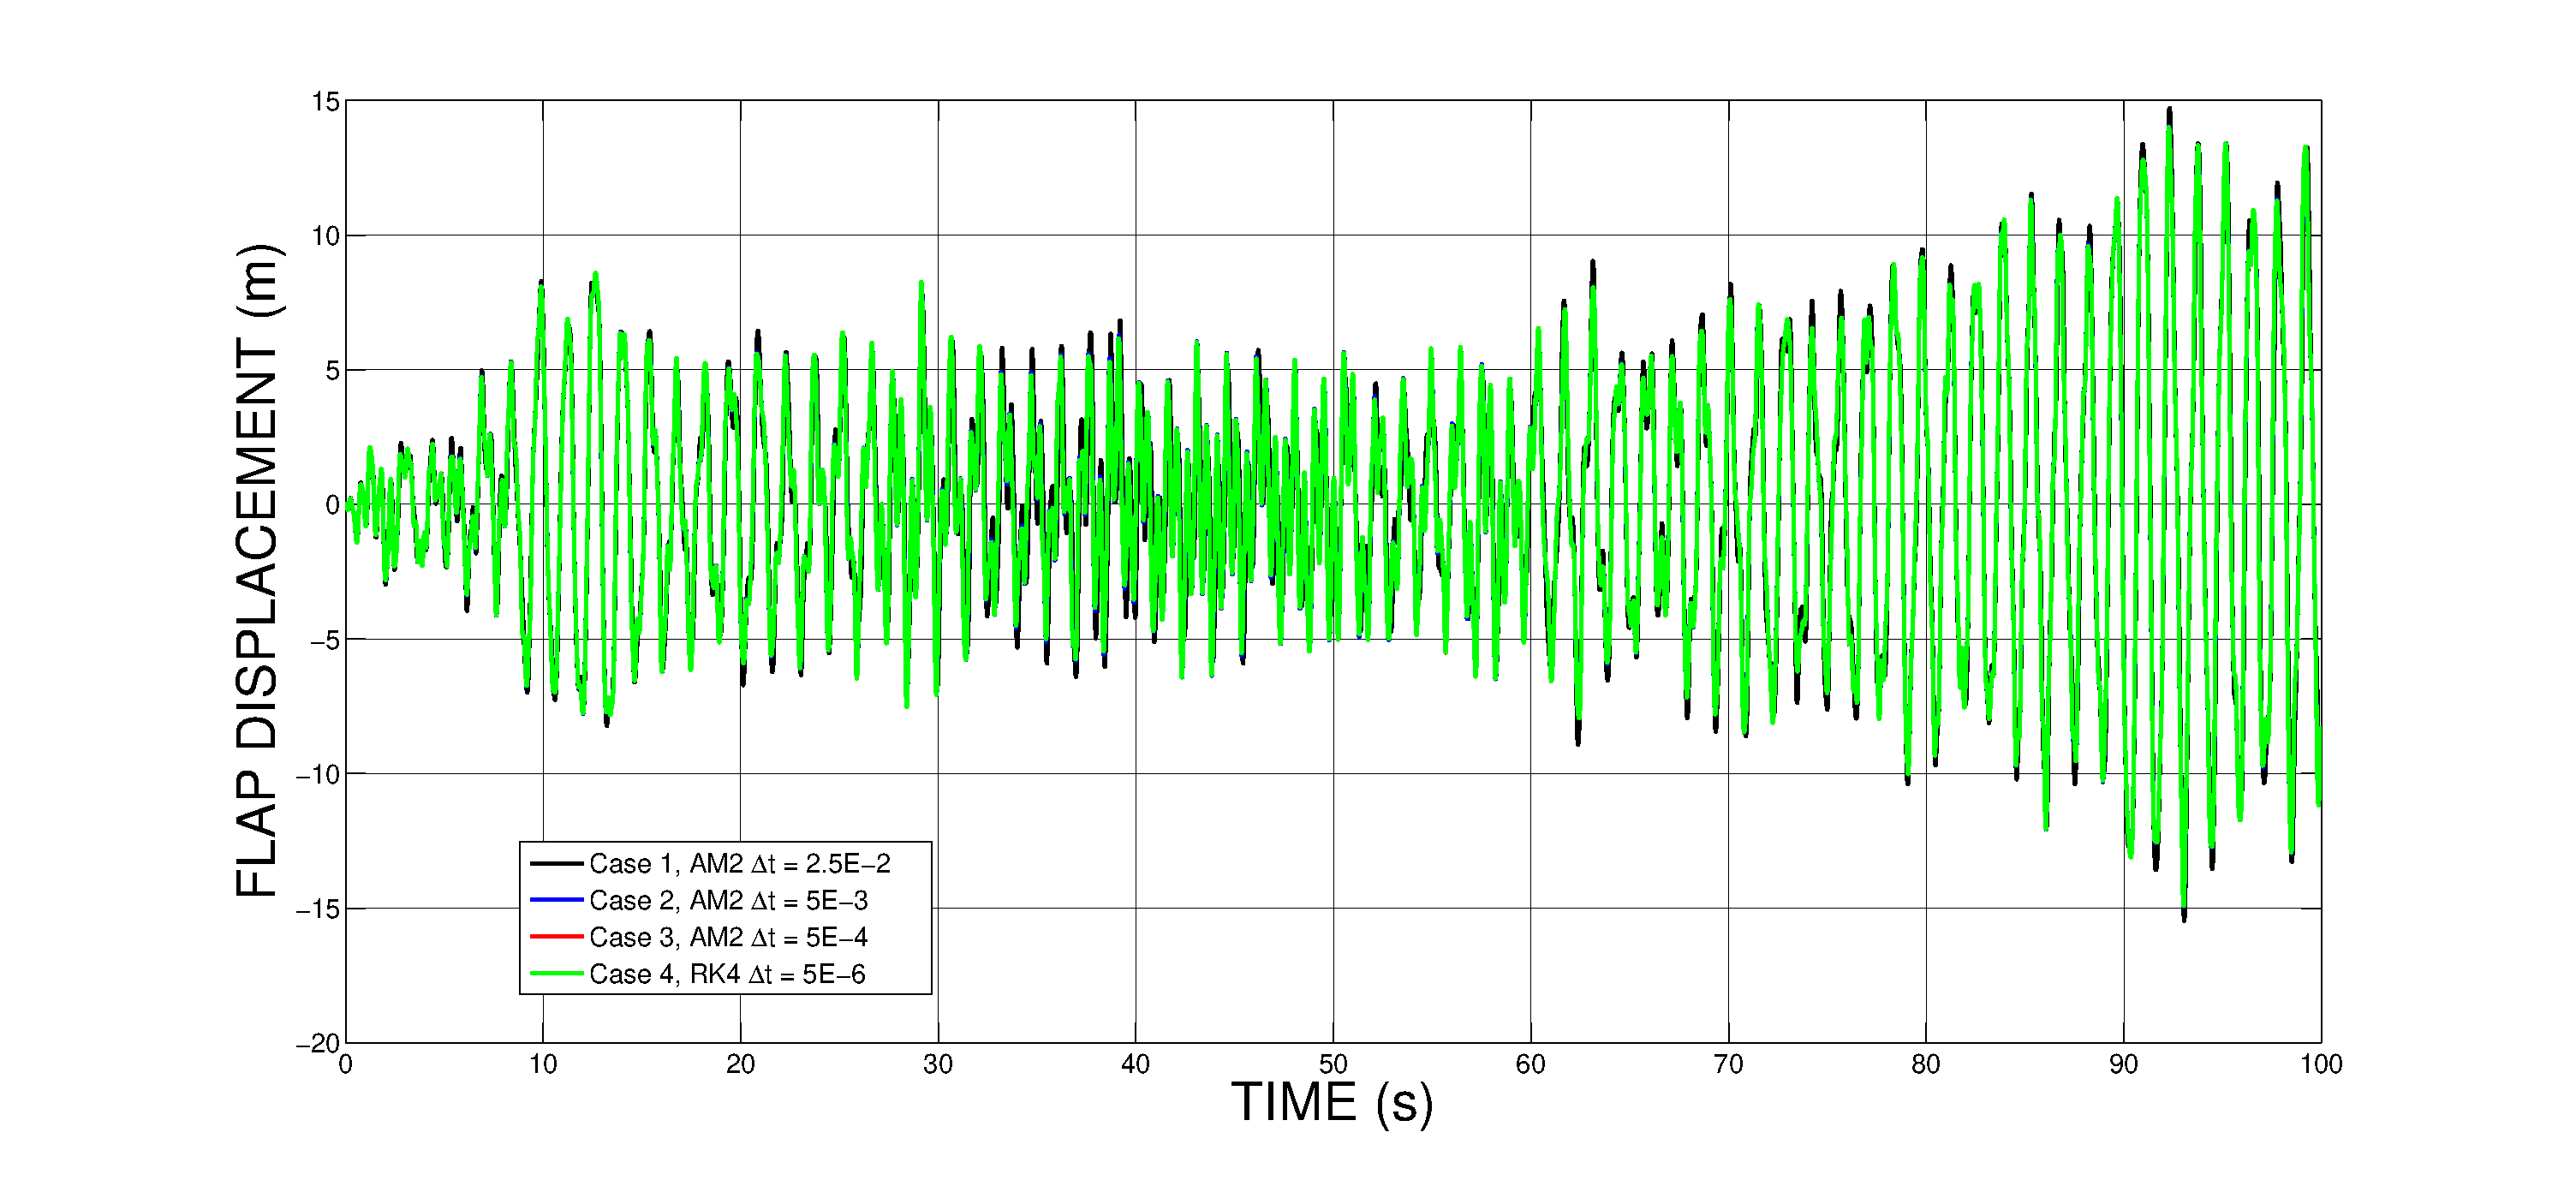
\includegraphics[width=2.2in]{EPSF/u_5MW_flap_final.eps}
     \end{center}
     
     \column{2.0 in}
    \pause
    \item PSD of Flapwise Response
    \begin{center}
     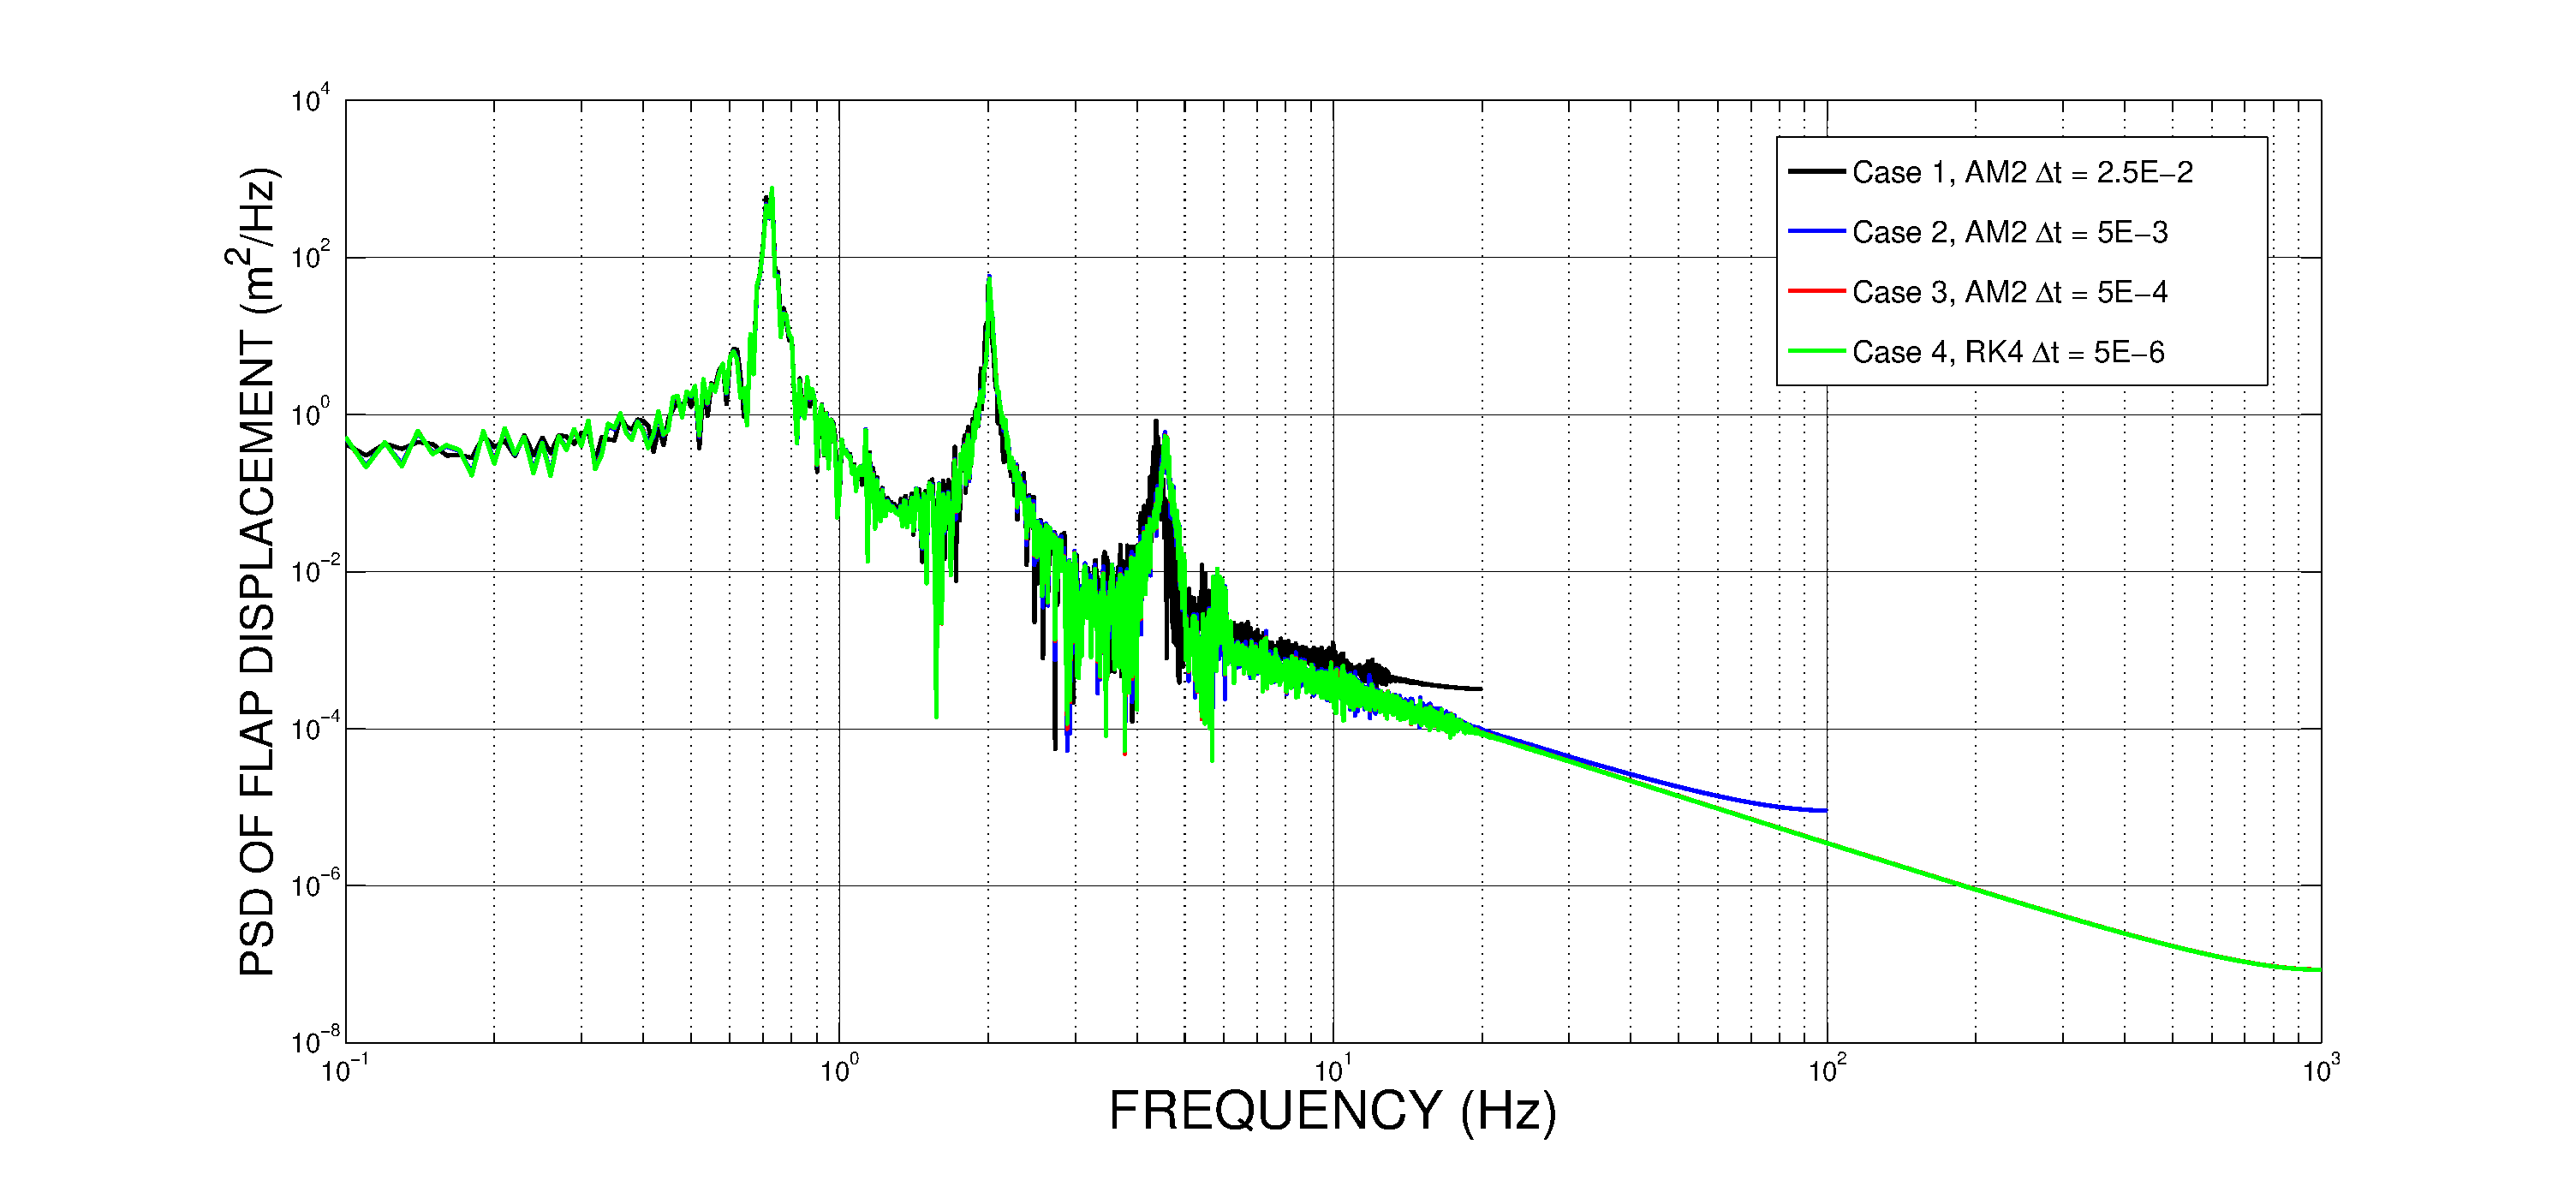
\includegraphics[width=2.2in]{EPSF/u_5MW_flap_psd_final.eps}
     \end{center}
     
     \end{columns}
     \begin{itemize}
        \pause
        \item For an implicit AM2 time step beyond 0.005 s, the solution is nearly identical to the fully resolved explicit RK4 solution
        \pause
        \item For an AM2 time step of 0.025 s, the solution remains stable and tracks the other solutions, but error grows at higher frequencies
        \pause
        \item The spikes at 0.7 Hz and 2 Hz correspond to the first and second blade flapwise natural frequencies
        \pause
        \item The spike above 5 Hz--above the frequency range of excitation--is brought about by nonlinear effects
     \end{itemize} 
\end{itemize}
\end{frame}
%------------------------------------------------------------------------------

%------------------------------------------------------------------------------
\begin{frame}{Example 4: NREL 5-MW Blade (Continued)}
  \begin{itemize}
      \item Convergence Rate
      \begin{figure}
\centering
\includegraphics[width=3.0in]{\directory RMS_5MW.eps}
\caption{ Normalized RMS error of flapwise displacement histories as a function of time step size for AM2 time integrator. The dashed line shows ideal second-order convergence.} 
\label{RMS_5MW}
\end{figure}
  \end{itemize}
\end{frame}
%------------------------------------------------------------------------------

%------------------------------------------------------------------------------
\begin{frame}{Example 4: NREL 5-MW Blade (Continued)}
  \begin{itemize}
      \item Solver Statistics
      
      \begin{columns}[c]
      \column{2.0 in}
      \begin{figure}
\centering
\includegraphics[width=2.0in]{\directory TotalNR.eps}
\caption{ Total number of linear system solves.} 
\end{figure}

     \column{2.0 in}
      \begin{figure}
\centering
\includegraphics[width=2.0in]{\directory AveNR.eps}
\caption{ Average number of linear system solves per step.} 
\end{figure}
\end{columns}
  \end{itemize}
\end{frame}
%------------------------------------------------------------------------------

%------------------------------------------------------------------------------
\begin{frame}{Summary}
    \begin{itemize}
        \item Conclusion
        \begin{itemize}
        \item Based on \alert{geometrically exact beam theory}, BeamDyn is capable of dealing with \alert{geometric nonlinear} beam problems with arbitrary magnitude of displacements and rotations for both static and dynamic analyses
        \item Along with a preprocessor like PreComp or VABS, BeamDyn takes \alert{full elastic coupling effects} into account
  \item The governing equations are reformulated into \alert{state-space form}, thus, making it amendable into FAST for tight-coupling analysis
  \item The space is discretized by \alert{spectral finite elements}, which is a p-version finite element, so that \alert{exponential convergence rate} can be expected for smooth solutions
  \item \alert{Different time integrators} have been implemented in BeamDyn; users will have options based on their needs
  \item BeamDyn is implemented following the programming requirements (data structures and interfaces) of the \alert{FAST modularization framework}
        \end{itemize}
    \end{itemize}
\end{frame}
%------------------------------------------------------------------------------

%------------------------------------------------------------------------------
\begin{frame}{Summary (Continued)}
   \begin{itemize}
   \item Future Work
    \begin{itemize}
            \item Coupling BeamDyn to FAST
            \item Full-Turbine validation
            \item Enhancement of numerical performance
        \end{itemize}
   \end{itemize}   
\end{frame}
%------------------------------------------------------------------------------


\begin{frame}[t]{Questions?}
\tiny
\psline[linewidth=4pt,linecolor=white](-4.0,0.7)(20,0.7)

\vspace{-0.1in}
\footnotesize
\textbf{Acknowledgments}
\begin{itemize}

\item Funded by the U.S. Department of Energy under Contract No.\
DE-AC36-08-GO28308 with the National Renewable Energy Laboratory.

\item Support was provided through an NREL Laboratory Directed Research and
Development grant \textit{High-Fidelity Computational Modeling of
Wind-Turbine Structural Dynamics}

%\item Computing resources were provided through the NREL Computational
%Science Center, which is supported by US DOE EERE Contract
%\#DE-AC36-08GO28308.

\end{itemize}

\textbf{References}
\scriptsize
\bibliographystyle{elsarticle-harv}
%\bibliographystyle{plain}
\bibliography{references}

\end{frame}

\end{document}


